\documentclass{article}
\usepackage[T1]{fontenc}
\usepackage[utf8]{inputenc}
\usepackage[brazil]{babel}

\usepackage{graphicx}
\usepackage{listings}

\lstset{
    basicstyle=\ttfamily
}

\newcommand{\FANN}{{\lstinline"FANN"}}
\newcommand{\opencv}{{\lstinline"opencv"}}
\newcommand{\train}{{\lstinline"train"}}
\newcommand{\test}{{\lstinline"test"}}

\begin{document}

\title{
    INE5443 --- Reconhecimento de Padrões\\
    OCR usando redes neurais com backpropagation
}
\author{
    Tiago Royer --- 12100776
}

\maketitle

\section{Enunciado}

O objetivo é utilizar redes neurais com backpropagation
para identificar dígitos.
Nos foram dadas 10 figuras, cada uma com um dígito diferente.
Estas imagens podem ser visualizadas na figura \ref{digitos}.

\begin{figure}[h]
    \centering

    \fbox{
\includegraphics{../img/0.png}}
    \fbox{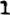
\includegraphics{../img/1.png}}
    \fbox{
\includegraphics{../img/2.png}}
    \fbox{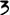
\includegraphics{../img/3.png}}
    \fbox{
\includegraphics{../img/4.png}}
    \fbox{
\includegraphics{../img/5.png}}
    \fbox{
\includegraphics{../img/6.png}}
    \fbox{
\includegraphics{../img/7.png}}
    \fbox{
\includegraphics{../img/8.png}}
    \fbox{
\includegraphics{../img/9.png}}

    \caption{Imagens que utilizamos para treinar a rede neural.}
    \label{digitos}
\end{figure}

\section{Implementação}

Para implementar as redes neurais, eu utilizei a biblioteca \FANN.
É uma biblioteca de redes neurais implementada em C.
Ela está disponível nos repositórios do Debian como o pacote \lstinline"libfann".

O \opencv foi utilizado para converter as imagens num vetor de pontos flutuantes.
Cada pixel virou uma entrada para a rede neural,
com valores entre 0.0 (branco) e 1.0 (preto).
Portanto, a rede neural possui 150 entradas.

A saída da rede neural codifica o valor da imagem na entrada em ``unário''.
Isto é, existem 10 nós na saída, cada nó correspondendo a um dos possíveis valores.

Eu fiz alguns testes com diferentes tamanhos para a camada interna.
Eu os descrevo na seção \ref{testes}.

\subsection{Interface com o usuário}

O código implementa, de fato, uma generalização da rede neural descrita acima.
Eu criei dois programas de linha de comando, \train\ e \test.
(O arquivo \lstinline"run.sh", no diretório raíz,
sumariza o ``pipeline de execução'' destes dois programas.)

O prgrama \train\ recebe, como parâmetro da linha de comando,
uma lista de imagens em escala de cinza,
e calibra uma rede neural para reconhecer estas imagens
conforme descrito na seção anterior.

Este programa escreve o resultado do treinamento da rede neural
no arquivo \lstinline"neural.net",
e os nomes dos arquivos utilizados no arquivo \lstinline"neural.data".

O programa \test\ lê estes dois arquivos e,
para cada imagem fornecida na linha de comando,
diz qual é o neurônio da camada de saída que ficou mais ativo
--- isto é, classifica a entrada.
(Na verdade, o programa escreve o nome do arquivo correspondente àquele neurônio.)

\section{Testes \label{testes}}

\end{document}
